%!TEX root = ../dissertation.tex
\section{Representation of eye orientation in 3 dimensions}
\label{cha2:represent}
In computer vision, it's customary to use the coordinate system on the left of Figure \ref{cha2:sec2:fig:coordsys2}, but in neuroscience a different convention, represented on the right of the Figure, is used. In order to be consistent with computer vision concepts, the former convention will be used throughout the remaining of this report.

\begin{figure}[!htb]
	\centering
	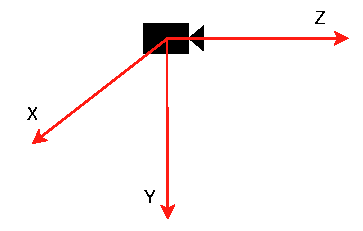
\includegraphics[width=0.41\textwidth]{images/cvcoordinatesys.pdf}
	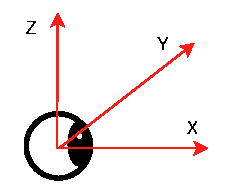
\includegraphics[width=0.25\textwidth]{images/cvcoordinatesysq.pdf}
	\caption[Computer Vision vs Neuroscience coordinate systems]{On the left, the right-handed coordinate system used in computer vision with the torsional component, Z, coming out of the front of the camera, the horizontal component as X and the vertical component as Y. On the right, the right-handed coordinate system used in the neuroscience field with the torsional component, X, coming out of the front of the eye, the horizontal component Y and the vertical component as Z. These last two components with an opposite direction in relation to the computer vision convention.}
	\label{cha2:sec2:fig:coordsys2}
\end{figure}

\subsection{Euler angles and Rotation matrices}
\label{rotmatsss}

A 3D rotation can be represented in several ways, the most common are Euler angles and rotation matrices. Euler angles are three angles that define three rotations applied successively to three axes. Considering two 3D orthogonal right-handed coordinate systems, their relative orientation can be described by a $3\times3$ rotation matrix, $R$, which is parameterized by the Euler angles. There are many axes sequence conventions for Euler angles, in this work the convention will be ZYX, which corresponds to rotating around the torsional, vertical and horizontal axes, respectively, according to the computer vision coordinate system in Figure \ref{cha2:sec2:fig:coordsys2}. In Figure \ref{cha2:sec2:fig:eulerangles}, it's shown a representation of this rotation. 
\begin{figure}[!htb]
	\centering
	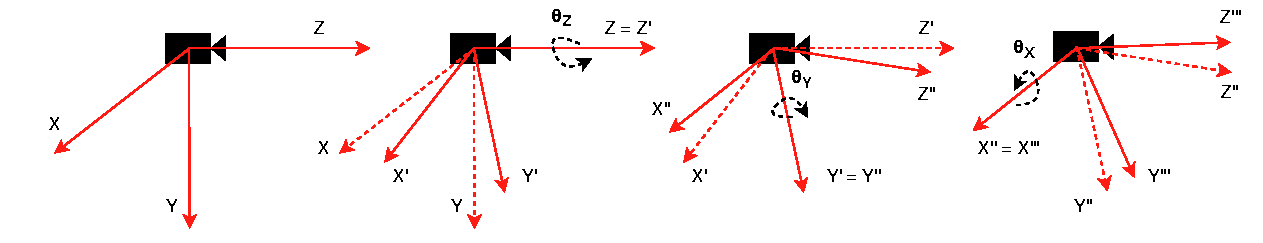
\includegraphics[width=\textwidth]{images/eulerangles.pdf}
	\caption[Euler angles convention ZYX]{From the left to the right, a sequence of counter-clockwise rotations around Z axis by $\theta_Z$, resulting in Z'Y'X', around Y axis by $\theta_Y$, resulting in Z''Y''X'' and around X axis by $\theta_X$, resulting in Z'''Y'''X'''. The coordinate system is right-handed.}
	\label{cha2:sec2:fig:eulerangles}
\end{figure}
The initial coordinate system is ZYX and the final coordinate system is Z'''Y'''X''', thus the rotation matrix can be defined as a multiplication (i.e. a serial order) of the following three rotation matrices, $R_Z$, $R_Y$ and $R_X$, noting that the order by which they are multiplied matters (rotations are non-commutative).
\begin{equation}
\label{rrr}
R _ { z } ( \theta_Z ) = \left[ \begin{array} { c c c } { \cos \theta_Z } & { - \sin \theta_Z } & { 0 } \\ { \sin \theta_Z } & { \cos \theta_Z } & { 0 } \\ { 0 } & { 0 } & { 1 } \end{array} \right], \
R _ { y } ( \theta_Y ) = \left[ \begin{array} { c c c } { \cos \theta_Y } & { 0 } & { \sin \theta_Y } \\ { 0 } & { 1 } & { 0 } \\ { - \sin \theta_Y } & { 0 } & { \cos \theta_Y } \end{array} \right], \
R _ { x } ( \theta_X ) = \left[ \begin{array} { c c c } { 1 } & { 0 } & { 0 } \\ { 0 } & { \cos \theta_X } & { - \sin \theta_X } \\ { 0 } & { \sin \theta_X } & { \cos \theta_X} \end{array} \right],
\end{equation}
A matrix originated from any combination of those is a rotation matrix when it satisfies the following conditions,
\begin{align}
	\label{epwifneprnf}
	R^{-1} = R^T\\
	\label{ienvpirnf}
	det(R) = 1.
\end{align} 

Instead of using multiple rotations done after each other around three different axes, Euler's theorem states that the orientation of the rotating body can also be parametrized by a single rotation with an angle, $\rho$, about an unitary axis in 3D, $\hat{\mathbf{n}} = (n_1, n_2, n_3)$. That rotation is denoted as $R(\hat{\mathbf{n}}, \rho)$ and is given by 
\begin{equation}
R ( \hat { \mathbf{n} } , \rho ) = \left( \begin{array} { c c c } { \cos \rho + n _ { z } ^ { 2 } ( 1 - \cos \rho ) } & { n _ { z } n _ { y } ( 1 - \cos \rho ) - n _ { x } \sin \rho } & { n _ { z } n _ { 3 } ( 1 - \cos \rho ) + n _ { y } \sin \rho } \\ { n _ { z } n _ { y } ( 1 - \cos \rho ) + n _ { x } \sin \rho } & { \cos \rho + n _ { y } ^ { 2 } ( 1 - \cos \rho ) } & { n _ { y } n _ { x } ( 1 - \cos \rho ) + n _ { y } \sin \rho } \\ { n _ { z } n _ { x } ( 1 - \cos \rho ) - n _ { y } \sin \rho } & { n _ { y } n _ { x } ( 1 - \cos \rho ) + n _ { z } \sin \rho } & { \cos \rho + n _ { x } ^ { 2 } ( 1 - \cos \rho ) } \end{array} \right).
\end{equation}

Still, rotation matrices are not the most efficient way to define rotations given they have nine elements and only three are actually necessary to describe the rotation uniquely. Hence, in oculomotor literature more suitable representations are used, such as quaternions, or rotation vectors that are more intuitive. \cite{rep}\cite{mathrot}

\subsection{Homogeneous coordinates}
\label{homo}
In computer vision, in order to facilitate calculations with rotation matrices and translation vectors, an extra dimension is added to the coordinates of a point. 
For a point $[x \ y]^T$, any three numbers, $[a_1 \ a_2 \ a_3]^T$ for which $\frac{a_1}{a_3} = x$ and $\frac{a_2}{a_3} = y$ are homogeneous coordinates. This three new coordinates are represented by "$\sim$", e.g. $\widetilde{a} = [a_1 \ a_2 \ a_3]^T$.


